\documentclass[pdf]{beamer}
\mode<presentation>{}
\usetheme{Dresden}
\usepackage{apalike}
\usepackage{graphicx}
\usepackage{subcaption}
\usepackage{pgfplotstable}
\usepackage{graphicx,psfrag}
\usepackage{amssymb}
\usepackage{mwe,tikz}\usepackage[percent]{overpic}
\usepackage{pifont}% http://ctan.org/pkg/pifont
\newcommand{\cmark}{\ding{51}}%
\newcommand{\xmark}{\ding{55}}%

%% preamble
\title{Dispersive Shock Waves of the Serre equations}
\author{Jordan Pitt, Stephen Roberts and Christopher Zoppou \\ Australian National University}
\newcommand\solidrule[1][0.25cm]{\rule[0.5ex]{#1}{1pt}}
\newcommand\dashedrule{\mbox{\solidrule[2mm]\hspace{2mm}\solidrule[2mm]}}
\newcommand{\dotrule}[1]{%
	\parbox[]{#1}{\dotfill}}

\begin{document}
%% title frame
\section{Introduction}
\begin{frame}
\titlepage
\end{frame}
\subsection{Introduction}

\begin{frame}{Introduction}
	Summary of our paper ``Behaviour of the Serre equations in the presence of steep gradients revisited" (Wave Motion Volume 76, January 2018). \newline \newline
	Outline of Presentation:
	\begin{itemize}
		\item Motivation.
		\item Serre Equations.
		\item Dispersive Shock Waves.
		\item Investigation.
		\item Results.
	\end{itemize}
\end{frame}

\begin{frame}<1>[label=BG]{Our Background}
	\begin{tabular}{l l l l}
		{ \color[RGB]{59,50,164} \usebeamertemplate{itemize item}{} } &Interest &:& Numerical methods for water waves \\ &&&focusing on ocean hazards. \\ \\
		\pause
		{ \color[RGB]{59,50,164} \usebeamertemplate{itemize item}{} } &Resulted In &:& Robust numerical method for the \\ &&& Shallow Water Wave Equations (ANUGA). \\\\
		\pause
		{ \color[RGB]{59,50,164} \usebeamertemplate{itemize item}{} } & Current Goal &:& Robust numerical method for the \\ &&& Serre equations.\\\\
		\pause
		{ \color[RGB]{59,50,164} \usebeamertemplate{itemize item}{} } &Problem &:& Handling discontinuous initial conditions \\ &&& (dam-break problem).
	\end{tabular}
\end{frame}

\begin{frame}{Indian ocean tsunami}
	\begin{figure}
		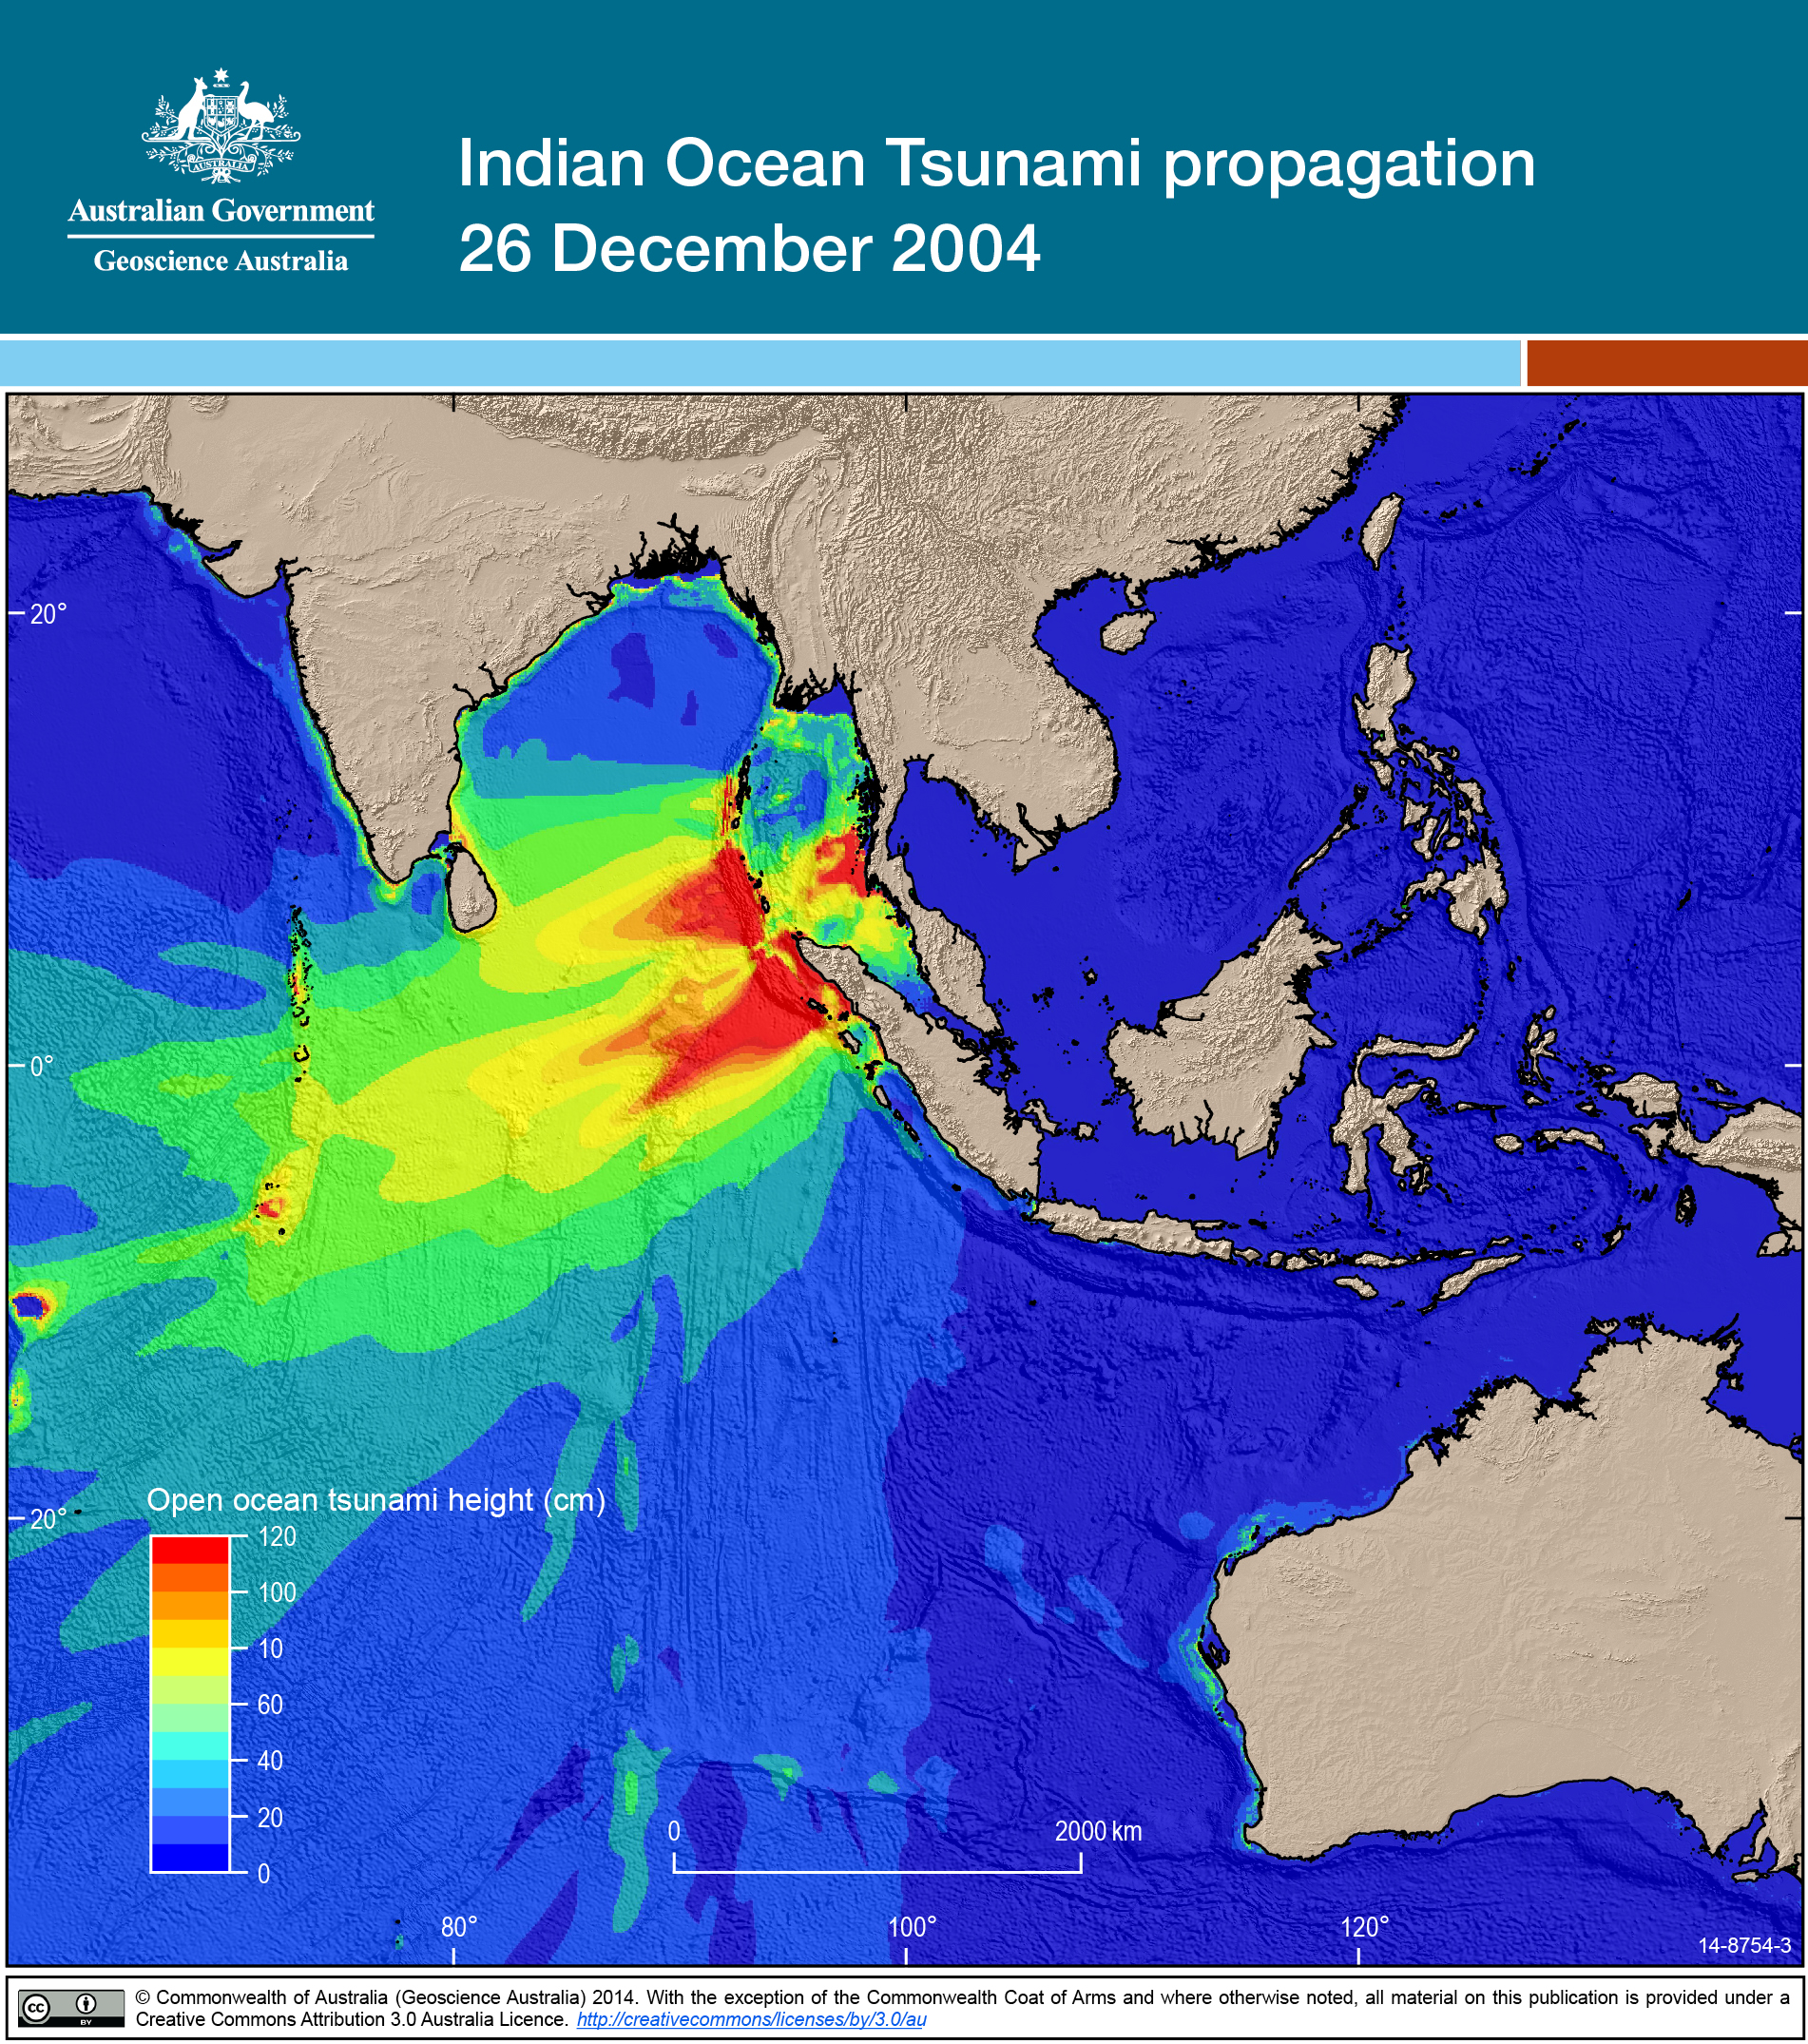
\includegraphics[width=5cm]{./Pictures/Introduction/IOT.jpg}
	\end{figure}
\end{frame}

\againframe<2>{BG}


\begin{frame}{Shallow Water Wave Equations}
	\hspace*{-1cm}%
	   	\begin{minipage}{.5\textwidth}
	   		\begin{figure}
	   			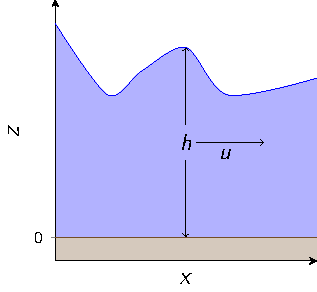
\includegraphics[]{./Pictures/Drawn/DepthAveraged.pdf}
	   		\end{figure}
	   	\end{minipage}%
	   	\hspace*{1cm}%
	   	\pause
   	\begin{minipage}{.5\textwidth}
   		Conservation of mass
   			\[
   			\dfrac{\partial h}{\partial t} + \dfrac{\partial (uh)}{\partial x} = 0
   			\]
   	    Conservation of momentum
   			\[
   			\dfrac{\partial (uh)}{\partial t} + \dfrac{\partial}{\partial x} \left ( u^2h + \dfrac{gh^2}{2}   \right )  = 0
   			\]
   	\end{minipage}
\end{frame}

\begin{frame}{Serre equations}

	Conservation of mass
	\[
	\dfrac{\partial h}{\partial t} + \dfrac{\partial (uh)}{\partial x} = 0
	\]
	
	Conservation of momentum
	\begin{equation*}
	\dfrac{\partial (uh)}{\partial t} + \dfrac{\partial}{\partial x} \left ( u^2h + \dfrac{gh^2}{2} + \dfrac{h^3}{3}{\color{red} \Phi }   \right )  = 0
	\end{equation*}
	
	\[ 	{\color{red} \Phi }  = \dfrac{\partial u }{\partial x} \dfrac{\partial u}{\partial x} -u \dfrac{\partial^2 u}{\partial x^2}  - \dfrac{\partial^2 u}{\partial x \partial t}  \]
\end{frame}

\againframe<3-4>{BG}


\section{Dispersive Shock Waves}
\subsection{Dispersive Shock Waves}

\begin{frame}{Model Problem : Dam Break Problem}
	
   	\begin{minipage}{.4\textwidth}
	\begin{subequations}
		\begin{gather*}
		h(x,0) = \left\lbrace \begin{array}{c c}
		h_1  & x \le x_0\\ h_0  & x > x_0 
		\end{array} \right. 
		\end{gather*}
		\begin{gather*}
		u(x,0) = 0
		\end{gather*}
	\end{subequations} 
   	\end{minipage}%
   	\begin{minipage}{.6\textwidth}
   		\centering
   		$h_0 = 1m$ , $h_1 = 1.8m$ and $x_0 = 500m$
	\begin{figure}
		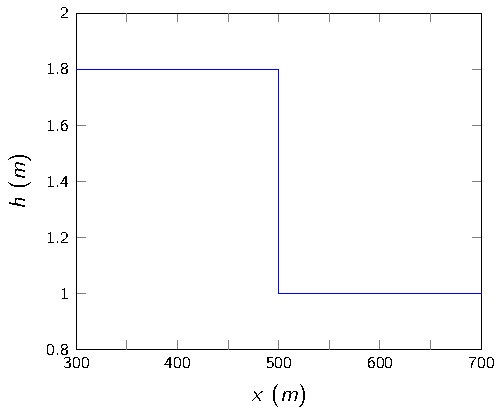
\includegraphics[width=1\linewidth]{./Pictures/DSW/DBinit.pdf}
	\end{figure}
   	\end{minipage}
	
\end{frame}

\begin{frame}{Dambreak Problem Solutions}
		
   \begin{figure}
    	\centering
    	\begin{minipage}{.5\textwidth}
    		\centering
    		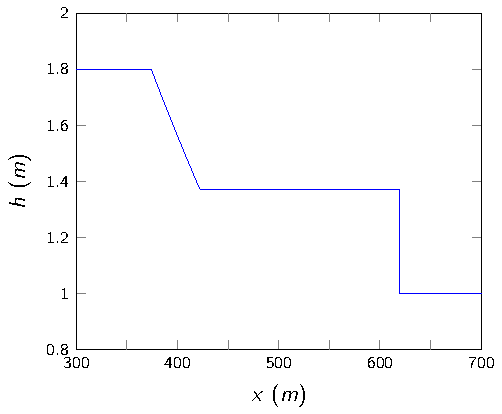
\includegraphics[width=0.95\linewidth]{./Pictures/DSW/SW.pdf}
    		\caption{Shock wave (analytical solution of the shallow water wave equations).}
    	\end{minipage}%
    	\pause
    	\begin{minipage}{.5\textwidth}
    		\centering
    		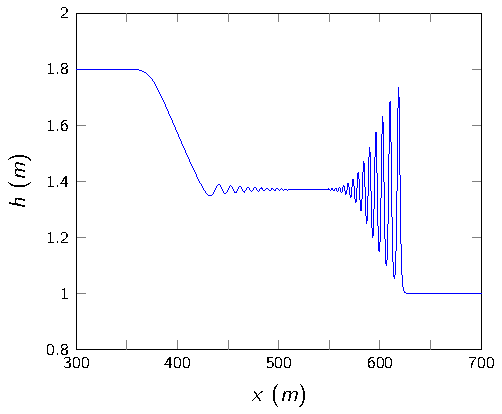
\includegraphics[width=0.95\linewidth]{./Pictures/DSW/DSW.pdf}
    		\caption{Dispersive shock wave (common numerical solution of the Serre equations in the literature).}
    	\end{minipage}
   \end{figure}
\end{frame}

\begin{frame}<1>{New Observed Behaviour for Dispersive Shock Waves}
	
	\begin{figure}
		\centering
		\begin{minipage}{.5\textwidth}
			\centering
			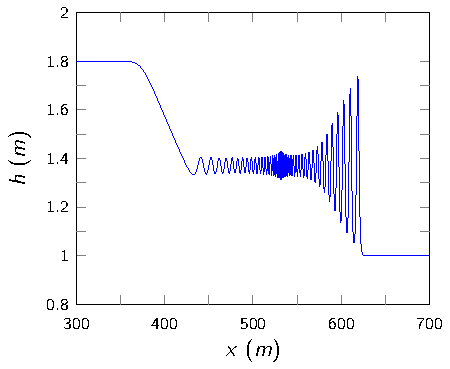
\includegraphics[width=1\linewidth]{./Pictures/DSW/DSWN1.pdf}
			\caption{New observed structure.}
		\end{minipage}%
		\pause
		\begin{minipage}{.5\textwidth}
			\centering
			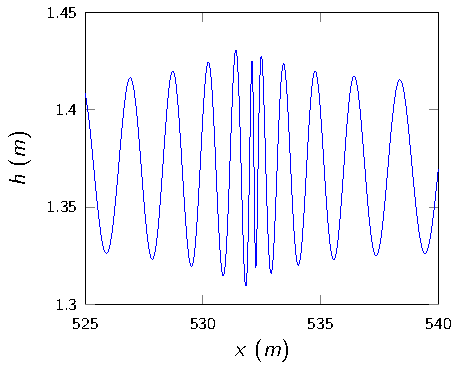
\includegraphics[width=1\linewidth]{./Pictures/DSW/DSWNz.pdf}
			\caption{Zoomed in.}
		\end{minipage}
	\end{figure}
\end{frame}

\begin{frame}{New Observed Behaviour for Dispersive Shock Waves}
	
	\begin{figure}
		\centering
		\begin{minipage}{.5\textwidth}
			\centering
			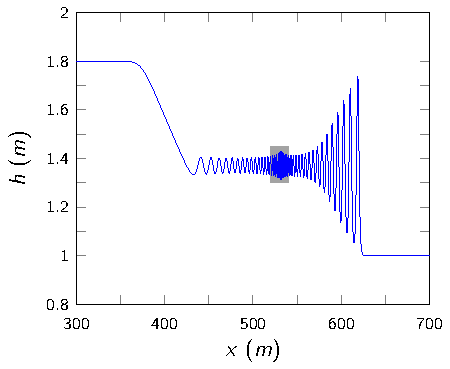
\includegraphics[width=1\linewidth]{./Pictures/DSW/DSWN2.pdf}
			\caption{New observed structure.}
		\end{minipage}%
		\pause
		\begin{minipage}{.5\textwidth}
			\centering
			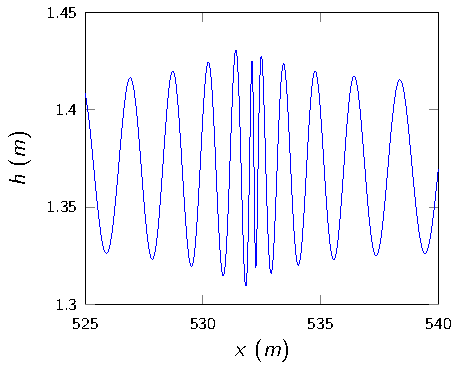
\includegraphics[width=1\linewidth]{./Pictures/DSW/DSWNz.pdf}
			\caption{Zoomed in.}
		\end{minipage}
	\end{figure}
\end{frame}



\begin{frame}<1>[label=test]{Properties of Dispersive Shock Waves of the Serre Equations}
	Asymptotic results for long times:
	\begin{itemize}
		\item Whitham modulation results for leading wave amplitude and location. \pause
		\item Oscillations of the dispersive shock waves for the Serre equations oscillate around the shock waves of the shallow water wave equations. \newline 
		\pause
	\end{itemize}
	Linear results:
		\begin{itemize}
			\item Separate dispersive wave trains.
		\end{itemize}
\end{frame}

\begin{frame}{Whitham Modulation Results}
		\begin{figure}
			\hspace*{-0.9cm}%
			\begin{minipage}{.5\textwidth}
				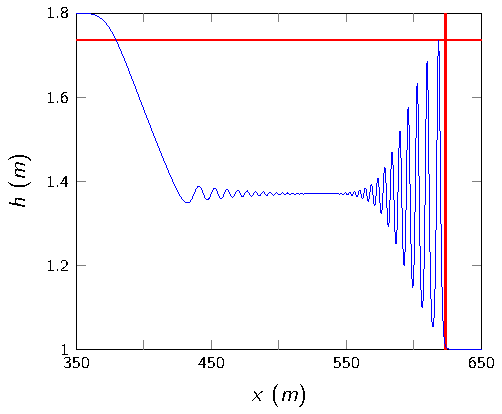
\includegraphics[width=1.2\linewidth]{./Pictures/DSW/DSWap.pdf}
				\caption{Common structure.}
			\end{minipage}%
			\hspace*{0.9cm}%
			\begin{minipage}{.5\textwidth}
				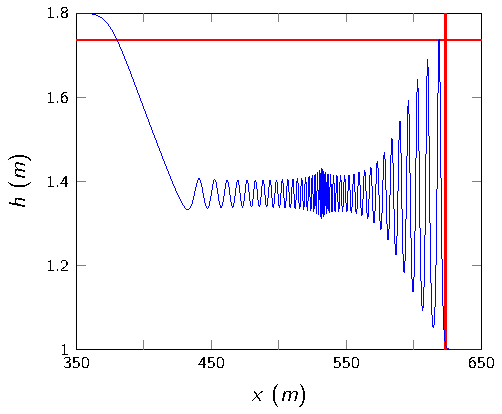
\includegraphics[width=1.2\linewidth]{./Pictures/DSW/DSWap1.pdf}
				\caption{New structure.}
			\end{minipage}
		\end{figure}
\end{frame}

\againframe<2>{test}

\begin{frame}{Dispersive Shock Waves compared to Shock Waves}
	\begin{figure}
		\hspace*{-0.9cm}%
		\begin{minipage}{.5\textwidth}
			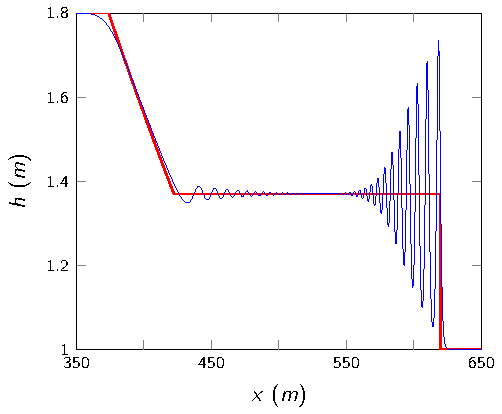
\includegraphics[width=1.2\linewidth]{./Pictures/DSW/DSWcompSW.pdf}
			\caption{Common structure.}
		\end{minipage}%
		\hspace*{0.9cm}%
		\begin{minipage}{.5\textwidth}
			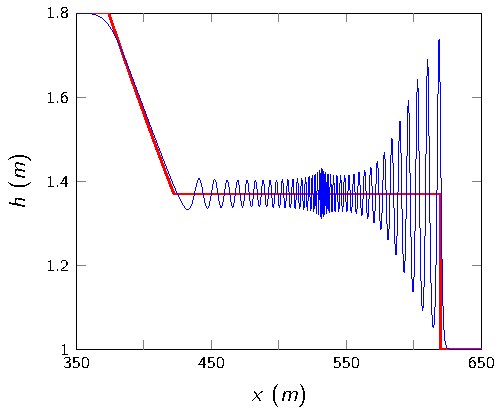
\includegraphics[width=1.2\linewidth]{./Pictures/DSW/DSWcompSW1.pdf}
			\caption{New structure.}
		\end{minipage}
	\end{figure}
\end{frame}

\againframe<3>{test}

\begin{frame}{Separation of Dispersive Wave Trains}
	\begin{figure}
		\hspace*{-0.9cm}%
		\begin{minipage}{.5\textwidth}
			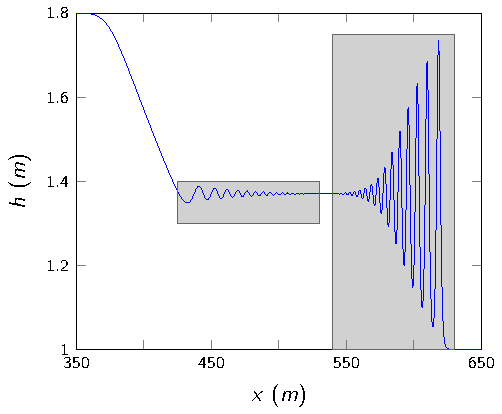
\includegraphics[width=1.2\linewidth]{./Pictures/DSW/DSWtails.pdf}
			\caption{Common structure.}
		\end{minipage}%
		\hspace*{0.9cm}%
		\begin{minipage}{.5\textwidth}
			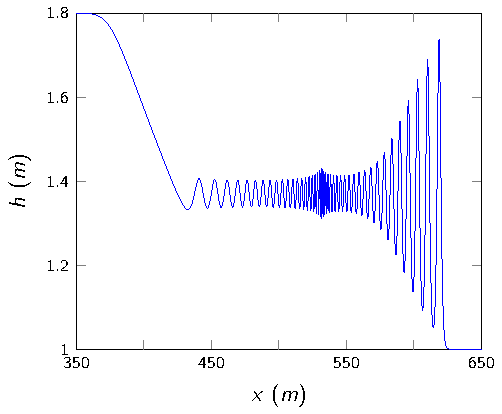
\includegraphics[width=1.2\linewidth]{./Pictures/DSW/DSWtails1.pdf}
			\caption{New structure.}
		\end{minipage}
	\end{figure}
\end{frame}


\begin{frame}{Problem}
	\begin{itemize}
		\item No analytic solution of the Serre equations for dispersive shock waves.
		\item Lack transient properties of dispersive shock waves.
	\end{itemize}
\end{frame}

\section{Investigation}
\subsection{Investigation}
\begin{frame}{Solution}
 	Use numerical solvers for the Serre equations on a problem with a smooth approximation to the initial conditions of the dam-break problem.
\end{frame}

\begin{frame}{Smooth Dam Break Problem}
	\begin{subequations}
		\begin{gather*}
		h(x,0) = h_0  + \frac{h_1 - h_0}{2} \left(1 + \text{tanh}\left(\frac{x_0 - x}{\alpha}\right)\right) 
		\end{gather*}
		\begin{gather*}
		u(x,0) = 0
		\end{gather*}
	\end{subequations} 
	\newline
	\centering
	$h_0 = 1m$ , $h_1 = 1.8m$ and $x_0 = 500m$
	
	
	
\end{frame}

\begin{frame}{Smooth Dam Break Problem Examples}
	\begin{figure}
		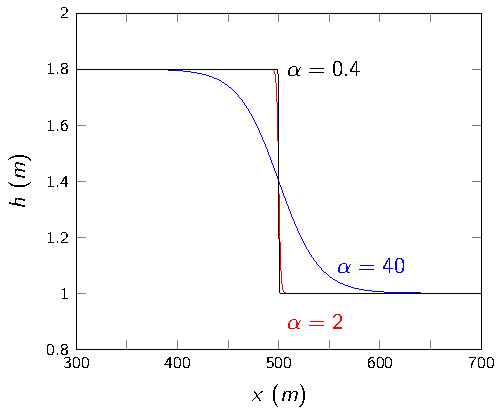
\includegraphics[width=0.7\linewidth]{./Pictures/DSW/DBSinit.pdf}
	\end{figure}	
	
\end{frame}


\section{Results}
\begin{frame}<1-2>[label=test12]{Observed Behaviours}
	We observed four different behaviours of the numerical solution as $\alpha \rightarrow 0 $
	\pause
	\begin{itemize}
		\item Non Oscillatory Structure for large $\alpha$ values.
		\pause 
		\item Flat Structure (common one in the literature).
		\pause
		\item Node Structure (also present in literature).	
		\pause	
		\item Growth Structure for small $\alpha$ values and the dam-break problem (New behaviour).
	\end{itemize}
\end{frame}

\begin{frame}{Non Oscillatory Structure $\alpha = 40$}
		\begin{figure}
			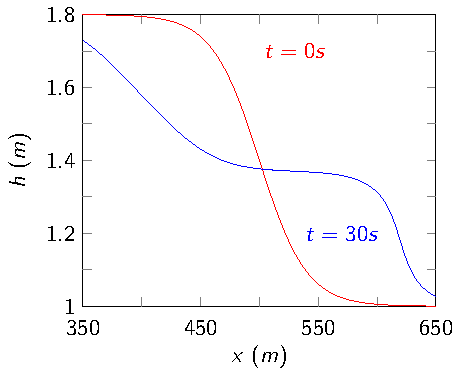
\includegraphics[width=0.65\textwidth]{./Pictures/Results/Example/non.pdf}
			\caption{Highest resolution numerical solution at $t=30s$}
		\end{figure}
\end{frame}

\againframe<3>{test12}

\begin{frame}{Flat Structure $\alpha = 2$}
	\begin{figure}
		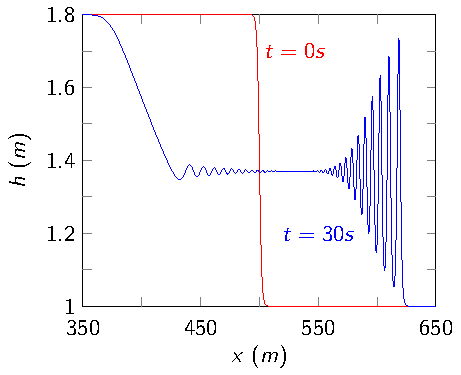
\includegraphics[width=0.65\textwidth]{./Pictures/Results/Example/flate.pdf}
		\caption{Highest resolution numerical solution at $t=30s$}
	\end{figure}
\end{frame}
\againframe<4>{test12}
\begin{frame}{Node Structure $\alpha = 0.4$}
	\begin{figure}
		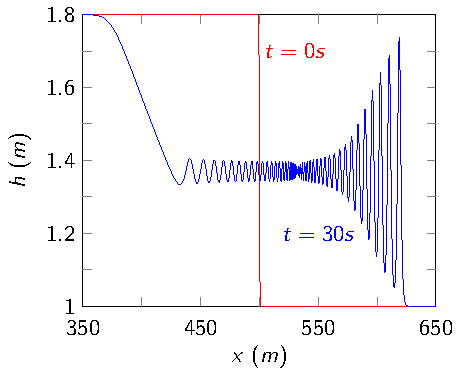
\includegraphics[width=0.65\textwidth]{./Pictures/Results/Example/node.pdf}
		\caption{Highest resolution numerical solution at $t=30s$}
	\end{figure}
\end{frame}

\begin{frame}{Node Structure $\alpha = 0.4$}
	\begin{figure}
		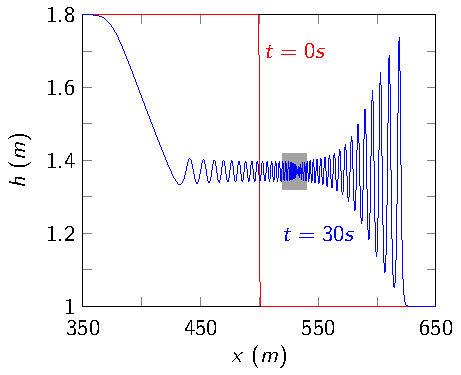
\includegraphics[width=0.65\textwidth]{./Pictures/Results/Example/node1.pdf}
		\caption{Highest resolution numerical solution at $t=30s$}
	\end{figure}
\end{frame}

\begin{frame}{Node Structure $\alpha = 0.4$}
	\begin{figure}
		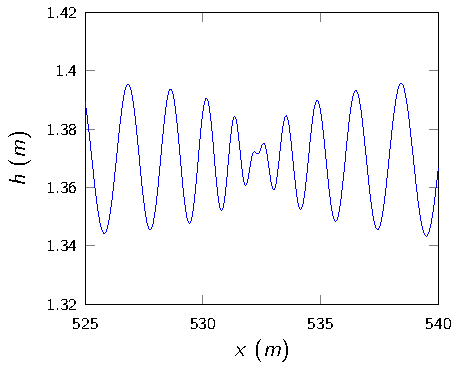
\includegraphics[width=0.65\textwidth]{./Pictures/Results/Example/nodez.pdf}
	\end{figure}
\end{frame}

\againframe<5>{test12}

\begin{frame}{Growth Structure $\alpha = 0.1$}
	\begin{figure}
		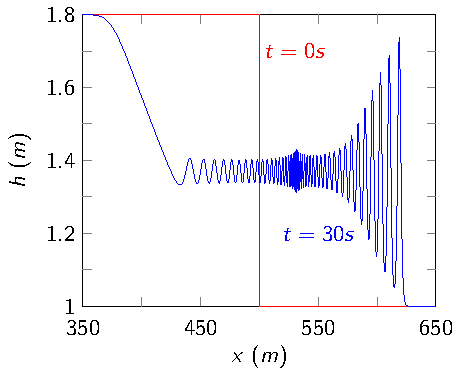
\includegraphics[width=0.65\textwidth]{./Pictures/Results/Example/growth.pdf}
		\caption{Highest resolution numerical solution at $t=30s$}
	\end{figure}
\end{frame}

\begin{frame}{Growth Structure $\alpha = 0.1$}
	\begin{figure}
		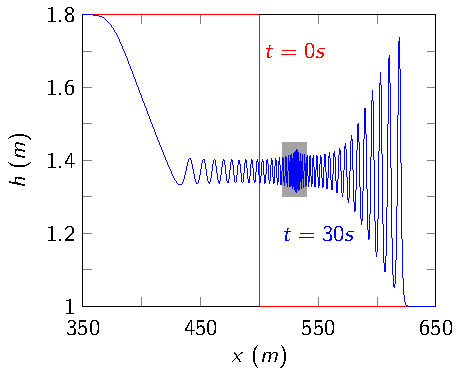
\includegraphics[width=0.65\textwidth]{./Pictures/Results/Example/growth1.pdf}
		\caption{Highest resolution numerical solution at $t=30s$}
	\end{figure}
\end{frame}

\begin{frame}{Growth Structure $\alpha = 0.1$}
	\begin{figure}
		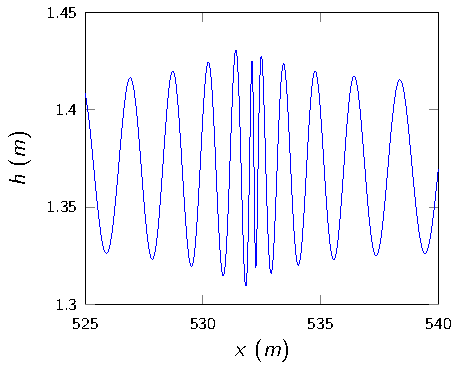
\includegraphics[width=0.65\textwidth]{./Pictures/Results/Example/growthz.pdf}
	\end{figure}
\end{frame}

\begin{frame}{Structure Comparison: Flat}
		\begin{figure}
			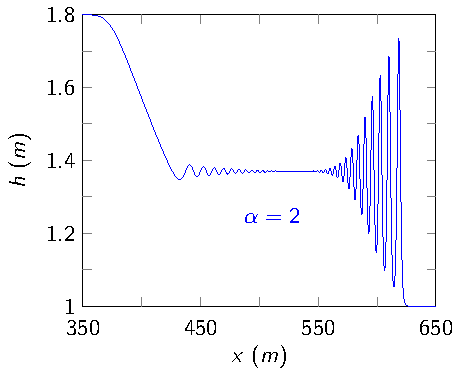
\includegraphics[width=0.7\textwidth]{./Pictures/Results/Example/6.pdf}
		\end{figure}
\end{frame}

\begin{frame}{Structure Comparison: Flat \& Node}
	\begin{figure}
		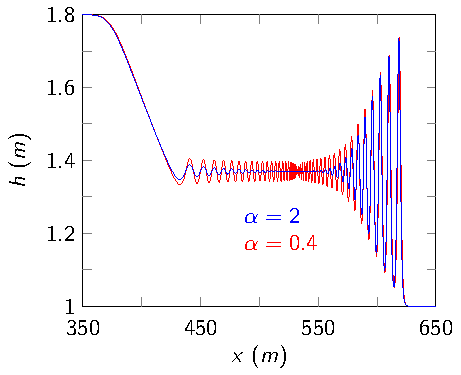
\includegraphics[width=0.7\textwidth]{./Pictures/Results/Example/69.pdf}
	\end{figure}
\end{frame}

\begin{frame}{Structure Comparison: Flat \& Node \& Growth}
	\begin{figure}
		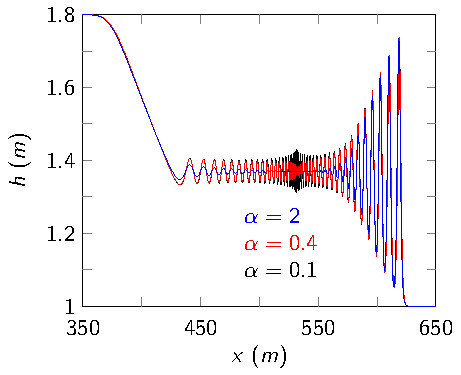
\includegraphics[width=0.7\textwidth]{./Pictures/Results/Example/6912.pdf}
	\end{figure}
\end{frame}

\begin{frame}{Structure Comparison Energy of Initial Conditions}
	Hamiltonian (Energy):
	\[\mathcal{H}(x,t) =\frac{1}{2} \left(hu^2 + \frac{h^3}{3}\left(\frac{\partial u}{\partial x}\right)^2 + gh^2\right) \]
	\newline 
	Comparison of Energy of Initial Conditions:
	\begin{center}
		\begin{tabular}{l | l | l}
			Structure & $\alpha$ & $\mathcal{H}$\\
			\hline
			Non-Oscillatory & $40$ & $10335.8$ \\
			Flat & $2$ & $10395.5$\\
			Node & $0.4$ & $10398.0$ \\
			Growth & $0.1$ & $10398.4$
		\end{tabular}
	\end{center}


\end{frame}

\begin{frame}{Justifying These Numerical Solutions}
	For a particular $\alpha$ value:
	\begin{itemize}
		\item Demonstrated convergence as the resolution of the method increases.
		\item Demonstrated numerical solutions conserve mass, momentum and energy.
	\end{itemize}
	These results demonstrated that the Growth Structure is correct structure of DSW for short time spans.
\end{frame}


\begin{frame}{Long term solutions}
	\begin{itemize}
		\item Growth structure agrees well with asymptotic results for short and long times.
		\item Growth structure decays to node structure which decays to the flat structure.
		\item Separation of dispersive wave trains over long times.
	\end{itemize}
\end{frame}

\begin{frame}{Dam break solution at $t=30s$ ($\alpha = 0$)}
		\begin{figure}
			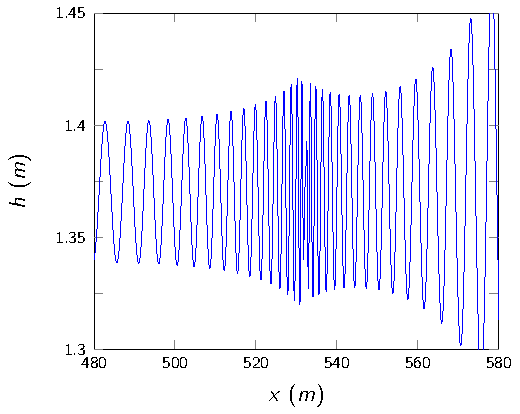
\includegraphics[width=0.65\textwidth]{./Pictures/Results/Example/G30.pdf}
		\end{figure}

\end{frame}

\begin{frame}{Dam break solution at $t=100s$ ($\alpha = 0$)}
	\begin{figure}
		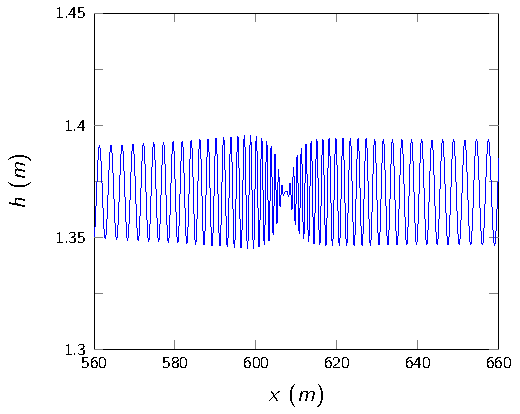
\includegraphics[width=0.65\textwidth]{./Pictures/Results/Example/N100.pdf}
	\end{figure}
	
\end{frame}

\begin{frame}{Dam break solution at $t=300s$ ($\alpha = 0$)}
	\begin{figure}
		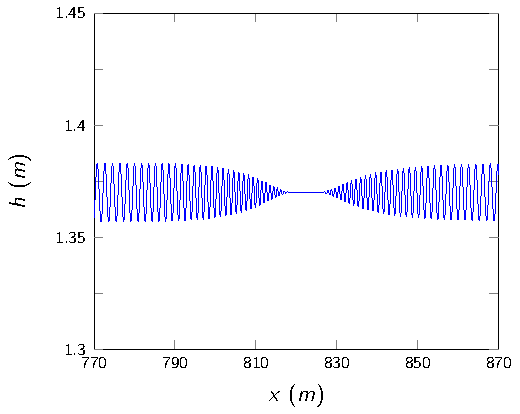
\includegraphics[width=0.65\textwidth]{./Pictures/Results/Example/F300.pdf}
	\end{figure}
	
\end{frame}



\begin{frame}{Conclusion}
	Presentation
	\begin{itemize}
		\item Found new behaviour of dispersive shock waves for short time spans not previously published in the literature.
		\item Good agreement between numerical solutions and known properties of dispersive shock waves for long time periods.
	\end{itemize}
	Paper
		\begin{itemize}
			\item Explained why different behaviour published in the literature.
			\item Justified the robustness of our numerical methods.
		\end{itemize}
\end{frame}

\begin{frame}{Comparison of Node and Growth Structures}
	\begin{figure}
		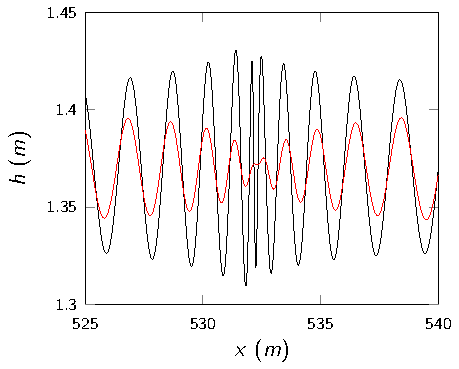
\includegraphics[width=0.7\textwidth]{./Pictures/Results/Example/912Comparison.pdf}
	\end{figure}
\end{frame}





\end{document}